\documentclass[twocolumn,floatfix,nofootinbib,aps]{revtex4-1}
\usepackage[utf8]{inputenc}

\usepackage{amsmath}    % need for subequations
\usepackage{amssymb}    % for symbols
\usepackage{graphicx}   % need for figures
\usepackage{verbatim}   % useful for program listings
\usepackage{color}      % use if color is used in text
\usepackage{subfigure}  % use for side-by-side figures
\usepackage{hyperref}   % use for hypertext links, including those to external
                        % documents and URLs
\usepackage[capitalise]{cleveref}   % use for referencing figures/equations
\usepackage{soul}

\begin{document}

\title{Optimal Parameter Selection in Markov State Models for Biomolecular Conformational Dynamics}
\author{Robert T. McGibbon}
\author{Christian R. Schwantes}
\author{Vijay S. Pande}

\begin{abstract}
Markov state models (MSMs) are a powerful tool for the analysis of molecular dynamics simulations, but have been hampered by the need for manual selection of the number of states. We report a new method for the optimal selection of the number of states in an MSM based on the Bayesian information criterion. We demonstrate the approach on three systems of increasing complexity...
\end{abstract}

\maketitle

\section{Introduction}
Protein are highly complex molecular machines, and their dynamics are an essential aspect of biomolecular function. These dynamics span a wide range of length scales, timescales and complexity, including folding and aggregation, conformational change between functional native substates, ligand binding, and allostery \cite{Dobson2003Protein, Kim2008Real, Austin1975Dynamics, Bahar2007Intrinsic}. Whereas classical experimental probes have often been interpreted in two-state frameworks, ensemble measurements with increasingly high temporal resolution as well as sensitive single molecule probes have uncovered a vast array of complex multi-state kinetics \cite{Cosa2006Evidence, Zhang2011Direct}. But the atomic-resolution characterization of these dynamics is often an enormous challenge -- as molecular probes like F\"{o}rster resonance energy transfer, small-angle x-ray scattering, and nuclear magnetic resonance techniques measure complex projections of the intrinsic structure, generally reporting simultaneously on many degrees of freedom\cite{Mertens2010Structural, Tzeng2011Protein}.

Computer simulations can complement experiments by providing atomic insight into conformational dynamics. With advances at the algorithmic, hardware, and software levels, modern molecular simulation paradigms, incorporating specialized or accelerated hardware, often in combination with highly parallel distributed computing frameworks, are capable of generating extensive simulation data sets\cite{Eastman2013OpenMM, Shirts2000Screen, Shaw2009Millisecond, Hess2008PLINCS, Buch2010High}. In fact, the minimally-biased kinetic analysis of such simulations is often a central bottleneck and presents a major challenge to the field. The analysis paradigms often entail the construction of lower resolution models parametrized from the high resolution simulation data set which capture the essential features in an interpretable framework\cite{Freddolino2010Challenges, Lane2013Milliseconds}. For example, by projecting the data down onto one or two degrees of freedom we create a simpler model for the system, such as one characterized by diffusion along a single reaction coordinate\cite{Best2010Coordinate}.

Markov state models (MSMs) are one approach for analyzing MD data sets and driving further MD simulations that are able to smoothly move between high and low-resolution models\cite{Pande2010Everything, Beauchamp2012Simple, Prinz2011Markov, Bowman2013Quantitative}. Such detailed models maintain quantitative agreement with the underlying simulation data, while low-resolution models capture the salient features of the potential energy landscape, sacrificing some degree of model complexity. In an MSM, the dynamics are modeled as a memory-less jump process between a discrete set of conformational states. The two key quantities which define the MSM are thus the state definitions, an indicator function basis over phase space, and the pairwise transition probabilities or transition rates, which parameterize the kinetics. The matrix of transition probabilities can be used to locate the systems transition paths\cite{Weinan2006Towards}, and its dominant eigenvectors to identify the metastable states\cite{Deuflhard2000Identification} and long-timescale dynamical modes\cite{}. 

A significant challenge in the automated construction of Markov state models is the choice of the number of states\cite{McGibbon2013Learning}. Although classical Hamiltonian dynamics form a continuous-time Markov chain in $\mathbb{R}^{6N}$, the Markov property does not hold after the projecting the dynamics onto a basis of discrete indicator functions. In particular, when states contain within them free energy barriers of substantial magnitude, the validity of the Markov assumption begins to suffer considerably. While this source of modeling error can be addressed by increasing the number of microstates, the reduction in one error comes at the expense of the increase in another. This second source of error is statistical in origin. As the number of states in the model grows, so does the number of parameters required to completely specify the kinetic model between all pairs of states. Because the amount of data is constant, each additional parameter leads to a decrease in the amount of data available per model parameter, which makes the approach susceptible to over-fitting.

Here, we seek to build models that are \emph{suitably} complex, given the data, yielding complex descriptions of the system only to the extent that their additional parameters are implied by the observed dynamics. To that end, we introduce a procedure for scoring the likelihood of an MSM, which, together with standard statistical model selection techniques, enables the optimal selection of the state space, which we express both in terms of the number of states and the clustering algorithm employed to group sampled conformations into states. This approach complements validation procedures performed primarily based on human intuition, such as Chapman-Kolmogorov tests, and enables the treatment of model selection as an optimization problem amenable to automated methods.

\section{Prior Work}
In the context of MSMs, model selection has traditionally been performed by analyzing the self-consistency of the models with respect to changes in the Markov lag time.

\begin{itemize}
\item Swope-Pitera http://pubs.acs.org/doi/abs/10.1021/jp037421y
\item Noe http://www.pnas.org/content/106/45/19011
\item Park and Pande
\item Sergio
\item Kellogg
\end{itemize}

After diagonalization of the transition matrix, the relaxation of any initial probability distribution can be described by a superposition of exponential relaxation processes, with a characteristic time given by $-\frac{1}{\ln \lambda_i}$.

\section{Likelihood of a Markov State Model}
With the kinetic model expressed as a set of pairwise state to state transition probabilities at a given lag time, the likelihood of an ensemble of trajectories after projection into the indicator function basis is given simply by the product of the transition matrix elements along the observed trajectories. However, as we vary the number of states, it is not permissible to simply compare these likelihoods as part of an optimization of the state definitions. In doing so, the optimal model would always be the trivial one state model, whose computed likelihood is unity regardless of the data.

The appropriate likelihood is instead a path action in phase space, on which the discrete states are merely an indicator function basis. With $s(X)$ as the function mapping conformations into the indicator function basis set, $s : \mathbb{R}^{3N} \rightarrow \{1, 2, \ldots, K\}$, the likelihood can be written as

\begin{align}
P[x_{0...T-1}] dx^T = \prod_{i=0}^{T-1} T(s(x_i) \rightarrow s(x_{i+1})) \cdot \prod_{i=0}^{T} p_{s(x_i)}(x_{i})
\label{eq:like}
\end{align}

With a discrete, non-overlapping state space, the likelihood of a sampled trajectory can be decomposed into a product of terms of two types: the state to state transition probabilities, $T(s_i \rightarrow s_j)$, and so-called emission distributions of each state, the conditional probability of observing a conformation at a given location in phase space given that the conformation, $x_t$ is within a certain state, $s(x_t)$.

For example, consider two Markov state models sharing the same transition matrix, $T$. In one model, the state emission distributions are highly peaked at specific locations in phase space, whereas in the other model the emission distributions are uniform over the volume of the states. If an observed trajectory does go through the first models' regions of high likelihood, it is appropriately termed a more likely model given the data.

This emission distribution can be potentially modeled in multiple ways, each of which, in combination with a transition matrix, parameterizes a different statistical model. We propose two possible distributions: first, one may model the conditional distribution $P(x_t | s(x_t))$ as a uniform distribution over the (hyper)volume of $s(x_t)$, as shown in eq. \ref{eq:like_vol}. This model has the advantage of appearing agnostic with respect to intra-state dynamics but is intractable in high dimensions when the states are defined by general polytopes, such as those produced by a data-driven Voronoi tessellation. A more tractable alternative is a Gaussian emission model where $P(x_t | s(x_t))$ is modeled as multivariate normal, where the pairwise overlap between the emission distributions is treated as a truncation error, as shown in eq.  \ref{eq:like_vol} and used in the popular X-means algorithm.\cite{Pelleg2000Xmeans} The truncation error steps from the fact that the emission probability distributions from every state assign nonzero probability to each conformation in a dataset, while the parameterization procedure for the Markov transition probabilities assumes each conformation to be uniquely assigned to a single state. Relaxing this approximation is possible with the forward-backward algorithm,\cite{Rabiner1989Tutorial} but is beyond the scope of this work.

%The simplest definition would be a uniform distribution since we are constructing an MSM that is agnostic to intra-state dynamics. When properly normalized, the uniform distribution takes a value of the reciprocal of the state's volume. This makes for an easy expression, however, volumes in high-dimensional states can be difficult to compute \ref{eq:like_vol}. For this reason, we can also choose other emission distributions that may be more tractable. In fact, \citet{Pelleg2000Xmeans} have used a gaussian emission distribution to define a likelihood to compare two k-means clusterings. The result of this emission distribution, is that the likelihood is proportional to the sum of square distances, which is precisely what is optimized in k-means clustering. If we think of k-centers as a poor man's version of k-means, then we can apply this same likelihood.

\begin{equation}
\label{eq:like_vol}
P[x_{0...T-1}] dx^T = \prod_{i=0}^{T-1} T(s(x_i) \rightarrow s(x_{i+1})) \cdot \prod_{i=0}^T \frac{1}{V_{s(x_{i})}}
\end{equation}

\begin{equation}
\label{eq:like_mvn}
\begin{split}
&P[x_{0...T-1}] dx^T = \prod_{i=0}^{T-1} T(s(x_i) \rightarrow s(x_{i+1})) \\
    &\cdot \prod_{i=0}^T \left(2 \pi\right)^\frac{d}{2} |\Sigma_{s(x_i)}|^{-\frac{1}{2}}  \exp\left(-\frac{1}{2} (x_i - \mu_{s(x_i)})' \Sigma_{s(x_i)}^{-1} (x_i - \mu_{s(x_i)})\right)
\end{split}
\end{equation}

where $\mu_{s(x_i)}$ is the cluster center assigned to $x_i$ and $\Sigma_{s(x_i)}$ is the corresponding covariance matrix. For simplicity, we follow \citet{Pelleg2000Xmeans} and employ a spherical Gaussian model with a single shared variance parameter across the states estimated by maximum likelihood, under which conditions eq. \ref{eq:like_mvn} reduces to
\begin{equation}
\label{eq:like_mvn2}
\begin{split}
P[x_{0...T-1}] & dx^T = \prod_{i=0}^{T-1} T(s(x_i) \rightarrow s(x_{i+1})) \\
	&\cdot \prod_{i=0}^T \left(2 \pi \hat{\sigma}^2\right)^{-\frac{d}{2}} \exp\left(-\frac{||x_i - \mu_{s(x_i)}||^2}{2 \hat{\sigma}^2}\right)
\end{split}
\end{equation} where
\begin{equation}
\label{eq:mle_sigma}
\hat{\sigma}^2 = \frac{1}{T - k} \sum_{i=0}^T || x_i - \mu_{s(x_i)} ||^2
\end{equation} where $k$ is the number of states.

\section{Cross Validation and the Bayes Information Criterion}

\begin{figure}
\centering
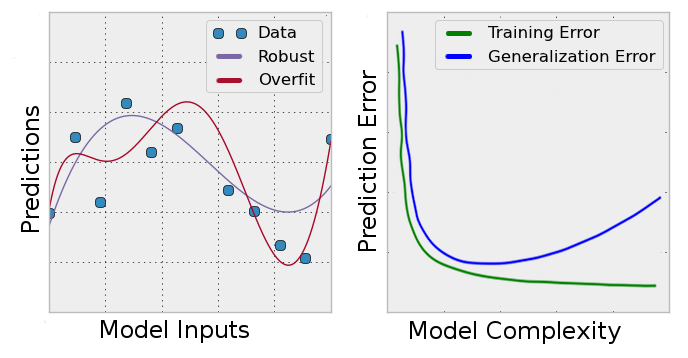
\includegraphics[width=3.1in]{figs/overfitting.png}
\caption{An example of overfitting. Left: in the presence of noise, a more complex model is able to fit the observed training data better, with lower residues and a higher empirical likelihood, but fails to distinguish the signal from the noise. Right: more complex model classes exhibit lower training errors, but generalize poorly to unobserved data.}
\end{figure}

Likelihood maximization is insufficient for model selection when the number of parameters varies between proposed models, as more complex models generally exhibit higher empirical likelihoods, often at the cost of larger generalization errors due to overfitting\cite{Liddle2007Information, Hastie01Elements}. Statistical learning theory provides a number of alternative approaches for this problem. Conceptually, the most straightforward is a full Bayesian treatment in which all unknown model parameters are represented by probability distributions. The evidence for a model is computed by formally integrating over the model parameters and the evidence ratio, or Bayes factor\cite{Gelfand94Bayesian}, then provides a rigorous basis of model selection that appropriately punishes overly complex models as they become poorly constrained in parameter space. Unfortunately such approaches are intractable for problems of this size because of the need to integrate over all possible Markov models of a given size.

Instead, we explore three alternative procedures: cross validation, Schwarz's Bayesian information criterion (BIC)\cite{Schwartz78Estimating} and the Akaike information criterion (AIC)\cite{Akaike1974AIC} for choosing the number of states in a Markov state model. In cross validation, we attempt to directly measure the Markov model's generalization error. We parameterize the model, building both the state space and transition matrix on a subset of the available molecular dynamics trajectories, but evaluate the likelihood on the left-out portion. The AIC and BIC are augmented likelihood function approaches which do not require leaving out portions of the available data during fitting, and instead employ asymptotic approximations to the Bayesian evidence to directly penalize models with additional free parameters.

\begin{equation}
\label{eq:bic}
\mathrm{BIC} \equiv -2\cdot \ln L + k \cdot \ln N
\end{equation}
\begin{equation}
\label{eq:eic}
\mathrm{AIC} \equiv -2\cdot \ln L + 2 \cdot k
\end{equation}

where $L$ is the likelihood, $k$ is the number of free parameters, and $N$ is the number of data points, assumed to be independent and identically distributed.

\section{Computational Methods}

\begin{figure}
\centering
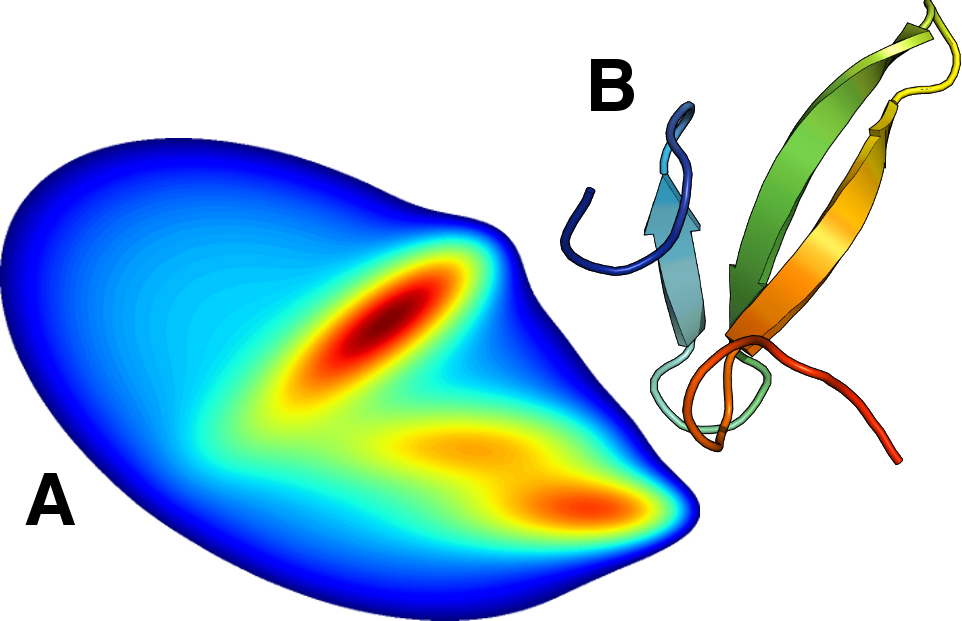
\includegraphics[width=3in]{figs/mull_ww.png}
\caption{Systems studied in this work. (A) Langevin dynamics on the two dimensional M\"{u}ller potential. (b) 200 $\mu s$ of dynamics of the Fip35 WW domain\cite{Liu2008Experimental}, courtesy of D.E. Shaw research \cite{Shaw2010Atomic}.}
\end{figure}

The uniform distribution emission model presents a computational challenge: its use requires the calculation of the (hyper)volume of the MSM's states, which, when defined by clustering are high-dimensional Voronoi cells. While trivial in two or three dimensions, this computational geometry task becomes challenging in high-dimensional settings. The computation of such volumes has occupied significant attention in recent years in the computational geometry literature, especially via randomized algorithms\cite{Kannan97, Simonovits03, Lovasz03}. We opt to approximate the volumes using naive Monte Carlo rejection sampling, which we find tractable for large systems only when the molecular dynamics dataset is first projected into a suitable small vector space of up to perhaps ten dimensions.

A further challenge is the procedure by which to model the volume of states which are at the edge of the MSM -- whose Voronoi cells extend to infinity in some direction. In these cases the Voronoi cells are of unbounded volume. Because the convex hull of our simulation datasets are computationally inaccessible, we define the outer extent of our data sets to be the set of all trial points such that the nearest sampled configuration to the trial point is closer than a certain cutoff, $R$.

For cross validation, we find it essential to use a dense prior during transition matrix estimation. Because the maximum likelihood transition matrix fit on a subset of the data assigns probability zero to unobserved transitions, we observe cross validation log likelihoods of negative infinity in all but the most data-rich regimes with maximum likelihood methods. For simplicity, we use the Jeffreys prior on each row of the transition matrix -- a Dirichlet prior with $\alpha=\frac{1}{2}$ -- which can be interpreted as a psuedocount of one half of an observed transition between each pair of states.

\section{Results and Discussion}
\subsection{M\"{u}ller Potential}
We simulated two trajectories with $10^6$ steps of Langevin dynamics on the M\"{u}ller potential\cite{}. Simulations were performed with a timestep $t=0.1$, friction coefficient of $\gamma=10^3$, and $kT=15$. The first trajectory was clustered using the $k$-centers clustering algorithm, and state volumes were computed for the uniform emission model using $10^5$ rounds of Monte Carlo rejection sampling with a padding distance of $R=0.2$ around the state centers from the 500 state model to define the dataset's envelope. The second trajectory was used as a test set.

The volumes did not change drastically upon doing ten times more Monte Carlo rejection sampling, and the likelihood remained essentially constant, which indicates that the use of approximation volumes is sufficient to obtain robust estimates of the likelihood. 

\begin{figure}[h]
\centering
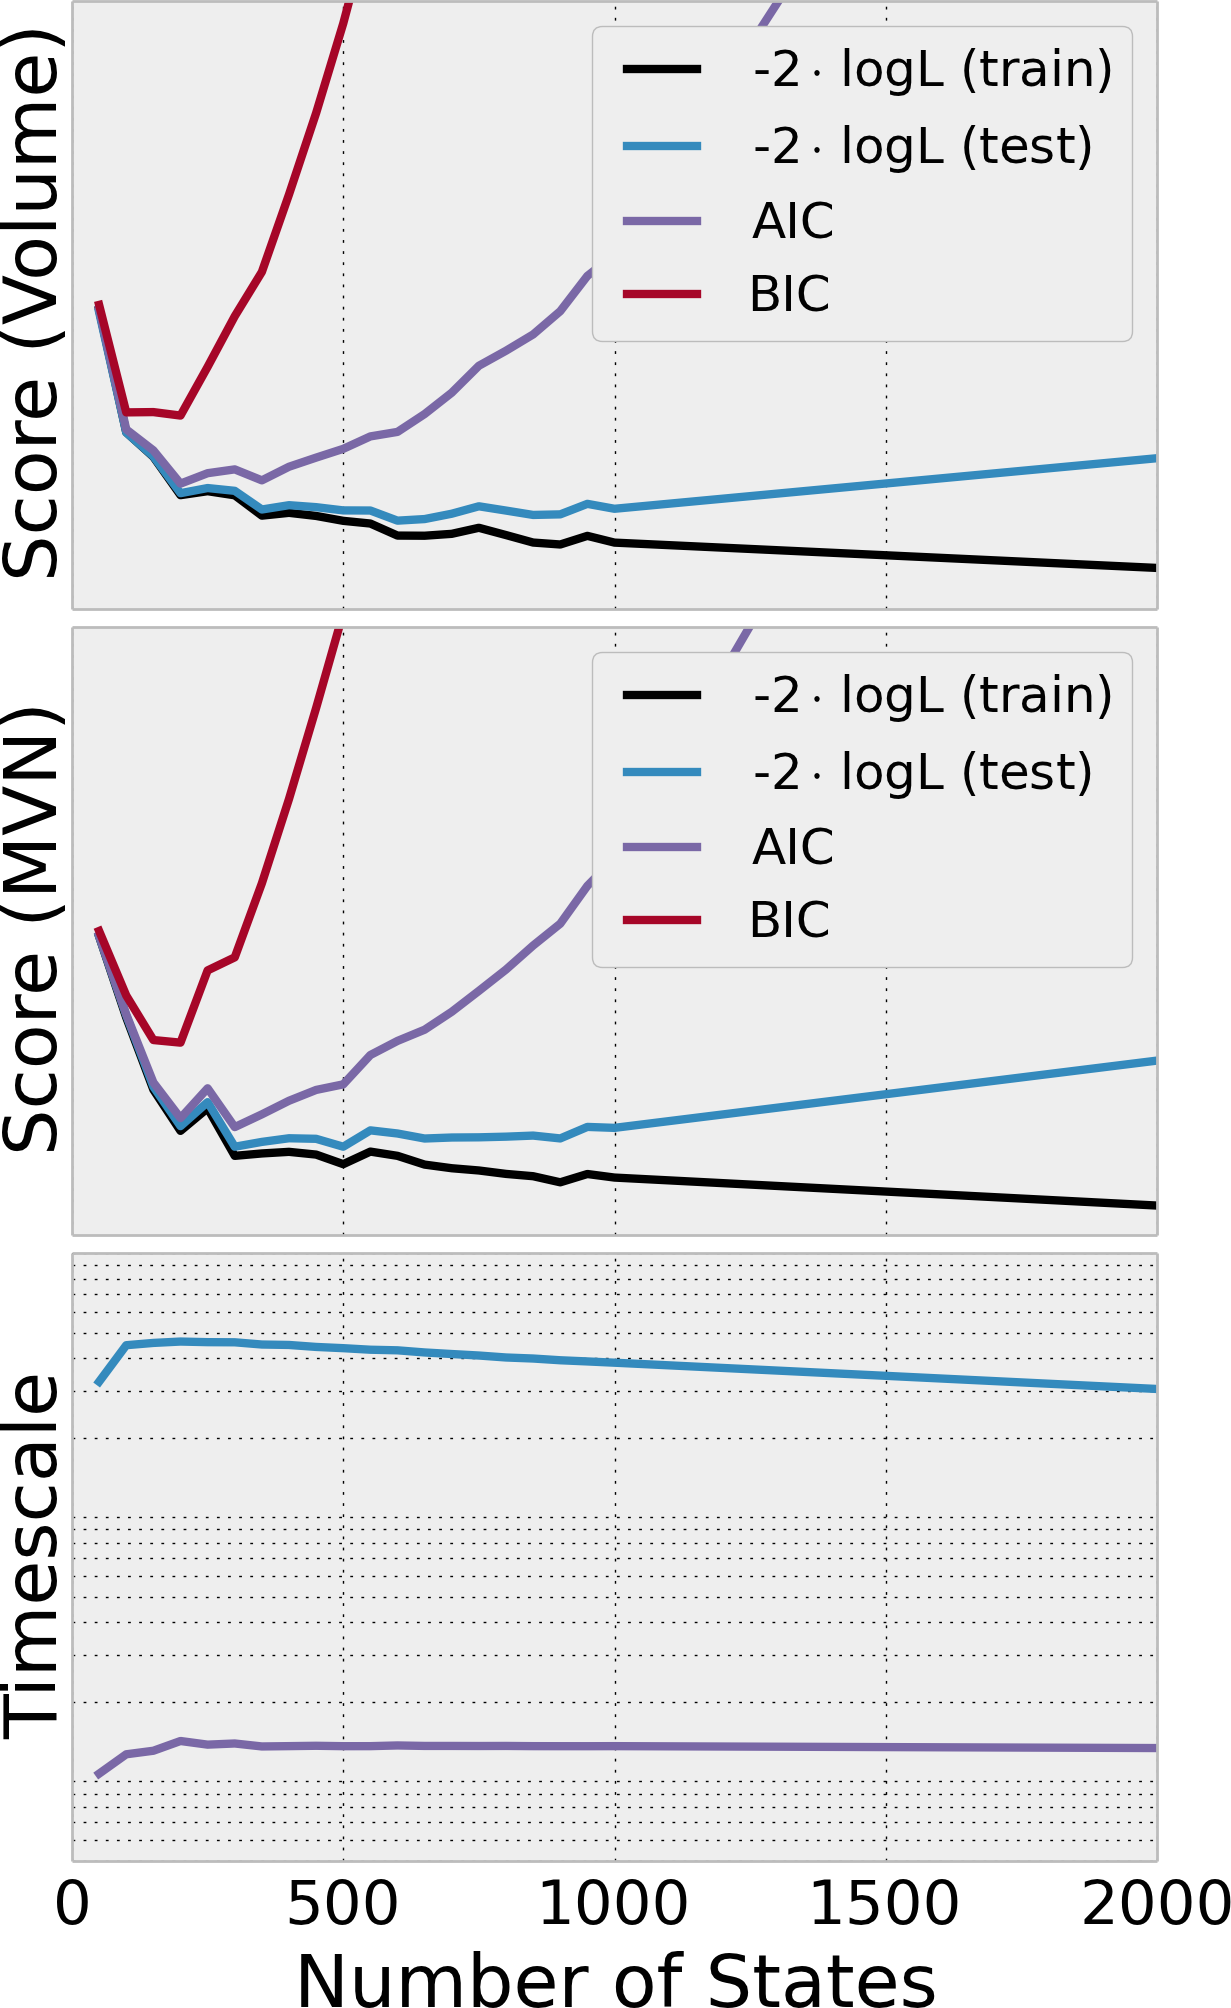
\includegraphics[width=2in]{figs/mull_cross_vert.png}
\caption{In models built using between 50 and 1,000 states with the $k$-centers algorithm, the log likelihood function increased quickly and plateaued at approximately 300 states. There are many methods that can be used to test the transferability of an MSM. We've plotted the AIC, BIC, and cross-validation scores for the M\"uller potential simulations. These results indicate that, at least for this dataset, the BIC and AIC may penalize the number of states too heavily.}
\label{fig:mullerlike}
\end{figure}

As shown in \cref{fig:mullerlike}, models built with too few states achieve a drastically reduced likelihood, but above a threshold region the likelihood increases relatively slowly. Here, the AIC and BIC's penalty on the number of parameters, which scales with the square of the number of states, begins to dominate. The optimal models according to the three methods are between 200 and 1000 states for this system. This observation is consistent with the convergence of the relaxation timescales of the models.

Interestingly, the AIC and BIC penalize the larger state models much more than the cross-validation approach. This could be due to the simplicity of this system. Since the M\"uller potential is only two-dimensional, it is difficult to actually produce a drastically over-fit model. We suspect that the cross-validation score on a real protein system would be closer to the BIC and AIC. However, we note, that cross-validation requires estimating a model without some subset of the data, which is not feasible for large systems in the data-sparse regime.

We also tested the Gaussian likelihood on MSMs built using k-means clustering on the M\"uller potential. The likelihood (\cref{fig:kmeans_mull}) peaks at a five-state model and decreases with the addition of further states. This maximum can be interpreted by inspecting the k-means cluster centers on the M\"uller potential. The five state model is the first model to have a cluster center located in the least stable well and as more states are added, the most stable well ends up being heavily split. We hypothesize that this over-splitting in the most stable minima gives rise to the decrease in MSM likelihood, and indicates a deficiency in clustering-based procedures which determine the state space without directly maximizing equations \ref{eq:like_vol} or \ref{eq:like_mvn}.

\begin{figure}
\centering
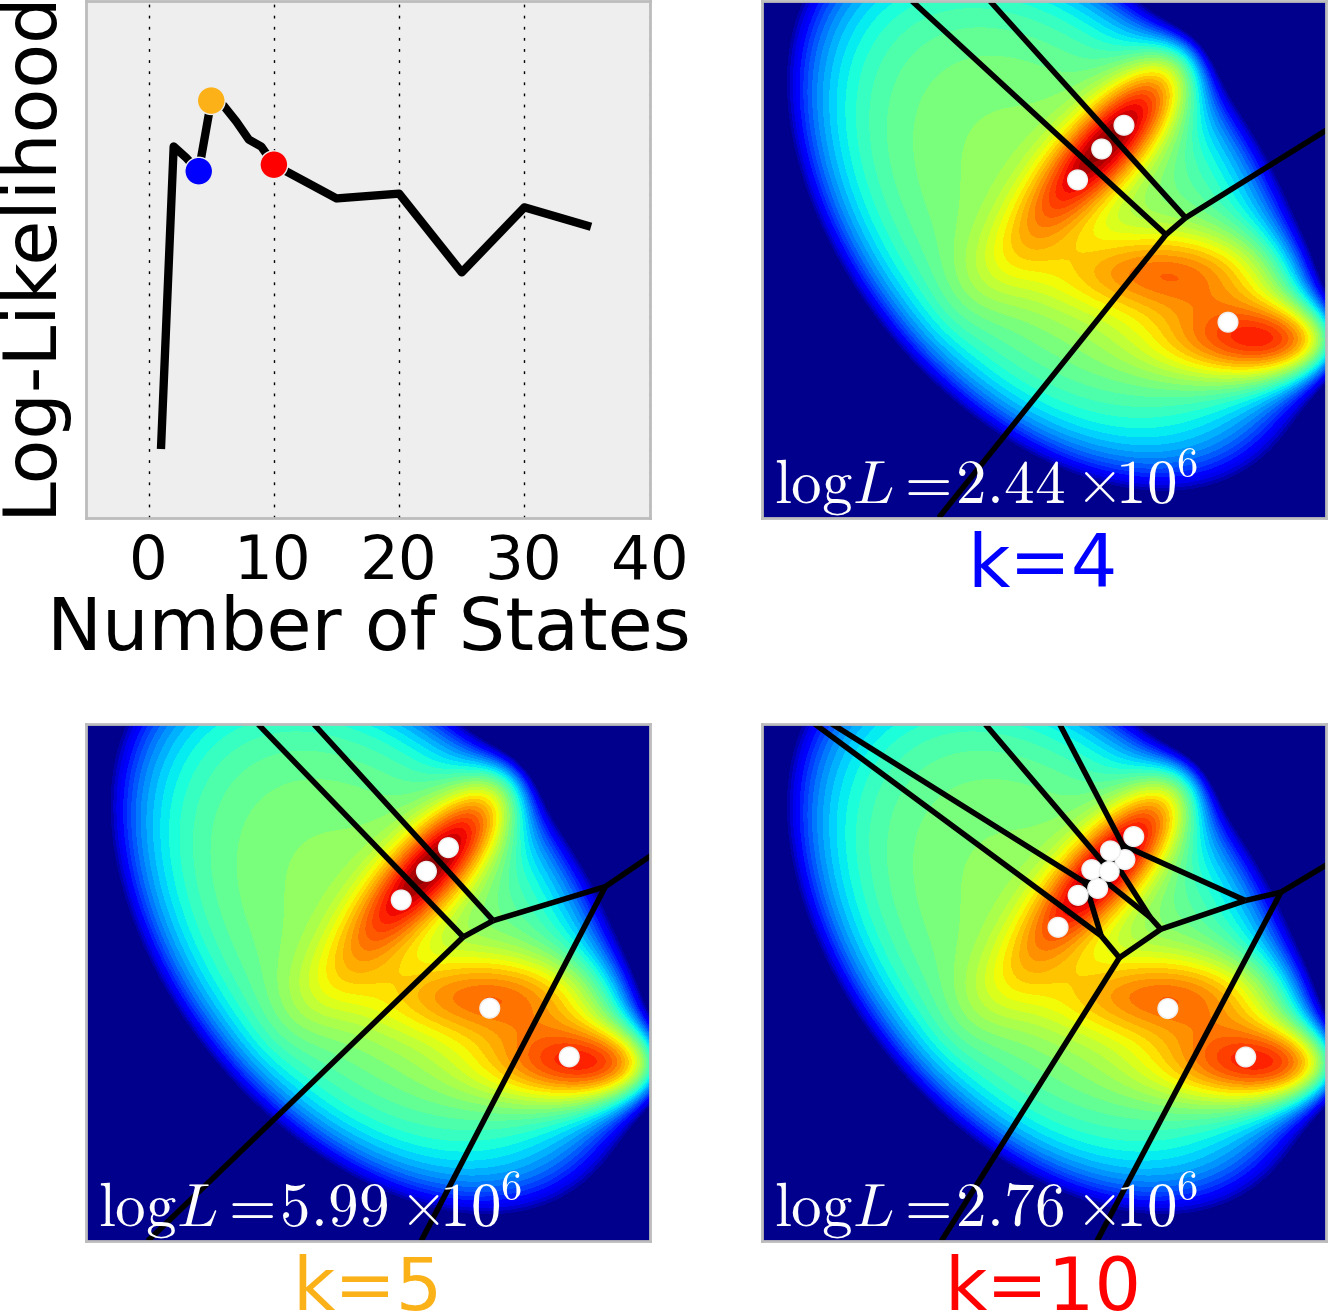
\includegraphics[width=3in]{figs/kmeans_vor_like.png}
\caption{MSMs were built using K-Means clustering on the M\"uller potential simulations. Since K-Means optimizes an objective function that is related to the emission probability, our likelihood picks only a few states as the most likely model. Interestingly, the likelihood decreases as you introduce additional states. This behavior is due to the state-to-state likelihood decreased rapidly when adding additional states, which may be a result of the large number of states in the most stable well.}
\label{fig:kmeans_mull}
\end{figure}

\subsection{Fip35 WW Domain}

To test the procedure on a larger protein system, we reanalyzed two ultra-long 100 $\mu s$ molecular dynamics trajectories of the Fip35 WW domain\cite{Liu2008Experimental}, provided courtesy of D.E. Shaw Research \cite{Shaw2010Atomic}. Because the likelihood calculations involving the uniform distribution emission model have exponential complexity in the dimensionality of the state space we first preprocess the trajectories with time-structure based independent components analysis (tICA) \cite{Schwantes2013Improvements, Perez2013Identification}, extracting only the the four slowest uncorrelated linear combinations of residue-residue distances. Using the Gaussian emission model, we compare both models built in the 3 dimensional tICA subspace and those built using k-centers clustering with the cartesian root-mean squared deviation (RMSD) over the Fip35 WW domain's 252 non-redundant heavy atoms, computed using the quaternion characteristic polynomial method\cite{Theobald2005Rapid}.

How many states are required in a Markov state model? The two 100 $\mu s$ molecular dynamics trajectories of the Fip35 WW domain simulated by Shaw et. al.\cite{Shaw2010Atomic} have been used to parameterize multiple Markov state models. \citet{Lane2011Markov} proposed a 26,000 state MSM after clustering the data by RMSD, whereas \citet{Kellogg2012Evaluation} clustering on contact maps, present a 1000 state model. We find the optimal number of states to be highly dependent on space in which the data is clustered. With RMSD, the Gaussian likelihood indicates that Markov models built with on the order of 5,000 states optimally balance model quality and generalization error. On the other hand, the tICA method's identification of slow order parameters in the simulations has the effect of reducing the number of states necessary when constructing Markov models: here we find high-quality models can be constructed using only on the order of 500 states. Even with 200-600 states, Markov models constructed using tICA are able to accurately identify the simulations folding process on the 1-10 $\mu s$ timescale, as well as the faster near-native dynamics identified in this dataset by \citet{McGibbon2013Learning}.

\begin{figure}
\centering
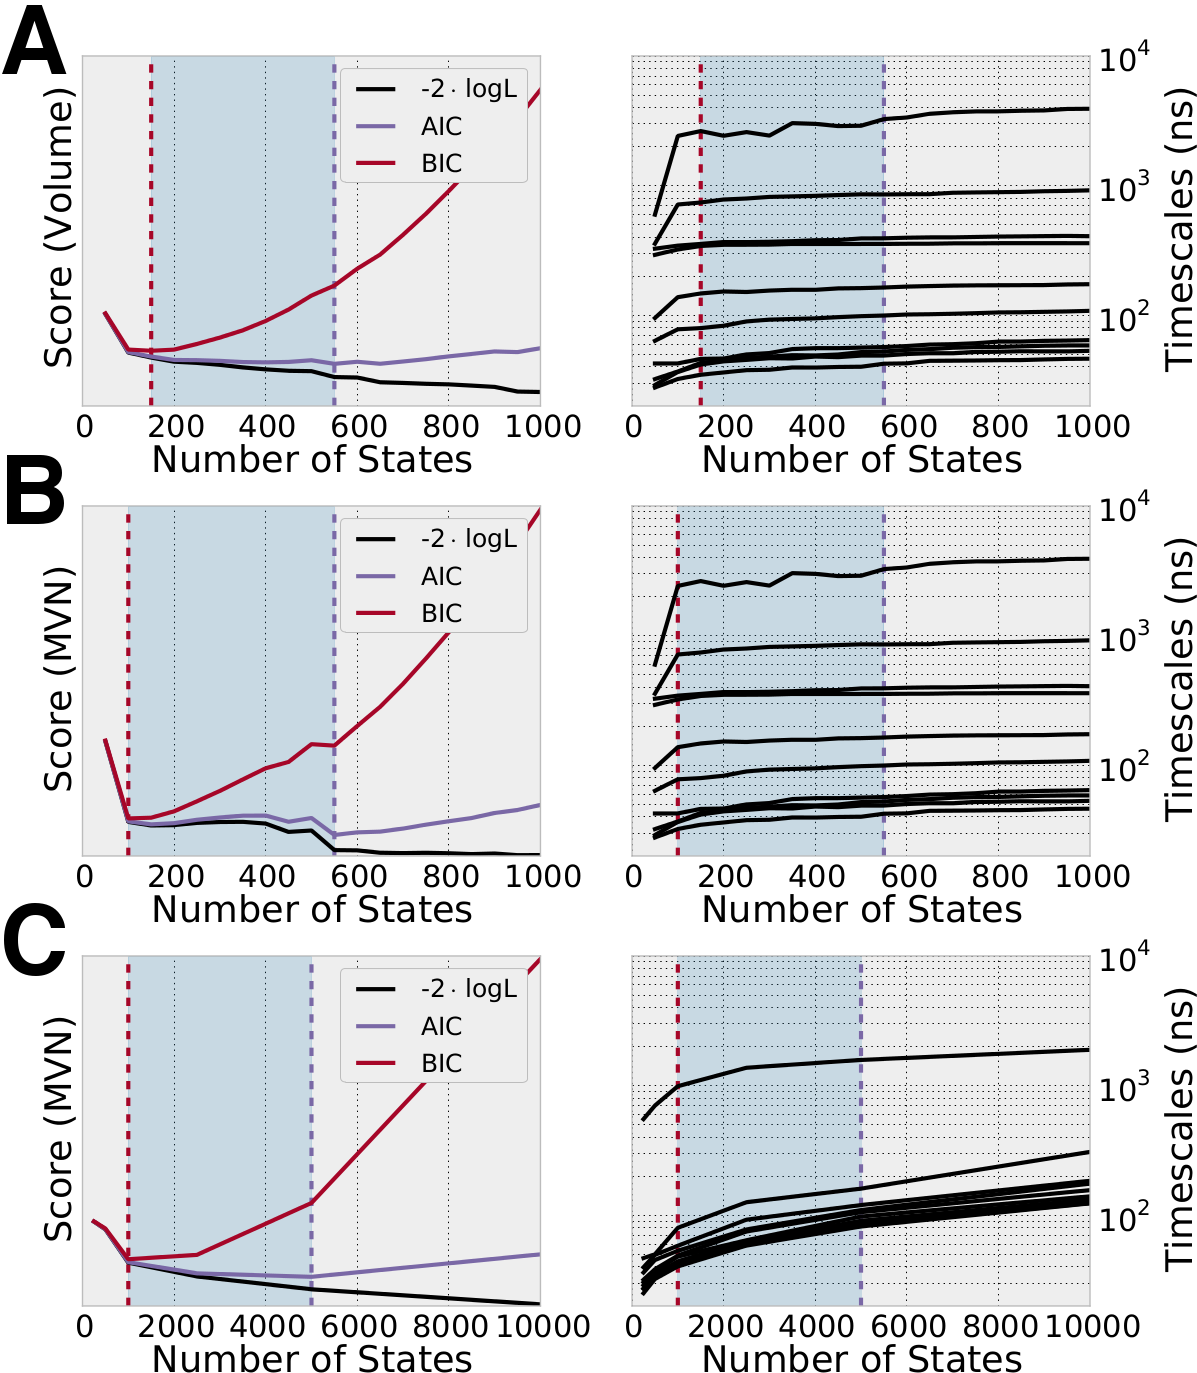
\includegraphics[width=3in]{figs/ww_logLs.png}
\caption{For models built using tICA, we were able to compute volumes as the dimensionality was low (A). These likelihoods were qualitatively similar to the MVN likelihoods (B). Because the MVN likelihood is easy to compute, we can use it to calculate the likelihood of a model clustered using the RMSD distance metric (C). Our likelihood indicates we should construct a model with 5000 states in the RMSD metric, whereas previous studies used a model with 26,000 states \cite{Lane2011Markov}.}
\label{fig:ww}
\end{figure}

\subsection{Limitations and Future Work}

The likelihood functions described herein permits the comparison of Markov state models with varying number of states, however it requires the definition of a vector space over which the emission model is defined. As such, models built on different projections of an underlying space cannot be directly compared. Furthermore, this approach is not amenable to optimizing the Markov lag time, the discretization interval for the Markov jump process. Nonetheless, we anticipate that automatic selection of the number of states in a Markov state model will remove much of the guess work in MSM construction, as the selection of the lag time is more amenable to existing Chapman-Kolmogorov tests.

In the future, we plan to extend this work to the consideration of models without discrete states, where the requirement that states strictly partition phase space into a set of discrete indicator functions is relaxed.

\section{Conclusions}

Markov State Models are powerful and popular tool for the analysis of molecular simulations, with a growing literature and two open source source software implementations\cite{Beauchamp2011Msmbuilder2, Senne2012EMMA}. There are, however a number of steps in the construction process that require human intervention, which limits the use of MSMs to experts and introduces significant biases into the model building process. Additionally, the ability to automatically construct Markov state models on the fly while simulations are in progress, an important point for so-called adaptive sampling procedures\cite{Bowman2010Enhanced}, is hampered when manual model selection is required. In the finite-data regime, additional complexity in the Markov model, in the form of increasing number of states, does come at a statistical cost.
These results take a step toward fully automating the MSM construction process and controlling this statistical error by providing a quantitative method for by which the most suitable discretization procedure can be selected.

\bibliography{bibliography}
\end{document}


\begin{itemize}
\item Is the 26,000 state model ``overfit''? The obvious answer, based on the line of reasoning that this paper is taking, is yes. But I think we need to consider the question a little more subtly. Perhaps it depends on what questions we ask of the model. When you ask both a ``properly-fit'' model and an overfit model a question that basically falls within the training set -- and neither of them need to extrapolate or really infer out-of-sample information, they'll both do fine. Heck, the overfit model might do better at telling you exactly what was \emph{in} the dataset.
\item The folding timescale is relatively insensitive to differences in MSM construction methodology. This has been observed in many datasets (McGibbon 2013, others). We hypothesize that this behavior is due to the large structural deviations at play -- even a two state model, given the same dataset, could basically get the right timescale just from counting the number of transitions. But finding these other timescales that are structurally subtle is different challenge. Also, how robust are other properties like experimental projections or the MFPT distribution to the number of states?
\item Single trajectory datasets are ``easier'' for MSMs. One of the uses of MSMs is to ``stitch together'' multiple trajectories -- this function only happens when the states are large enough that they \emph{connect} trajectories, so you can't have too many states in this case. But when you have a single trajectory, there's no possible way to create a disconnected model anyways.
\item We need to state, elegantly if possible, the differences between our likelihood and Liz Kellogg's. This requires some careful language, since we think there are methodological problems with her approach.
\end{itemize}




\begin{itemize}
\item This model doesn't help us pick the lag time.
\item It also doesn't help us pick the projected vector space, at least in a quantitative way. This is kind of a big deal, but it is what it is.
\item Uniform distributions are extremely inconvenient to work with. In the future, we plan to extend this work to Markov state models without discrete states.
\item \{I want to get this in print.\} Going forward, we anticipate that a combination of kinetic dimensionality reduction and clustering is going to be the key combination for robust Markov state model construction. The two approaches are characterized by complementary approximations and sources of error. In dimensionality reduction, the assumption is that the dynamics ``align'' with the vectors in some sense -- we talk about dynamics in the ``x direction'' as having some characteristic, regardless of whether they occur around $x=x_a$ or $x=x_b$. In clustering, if $x_a$ and $x_b$ are in different states, there's no crosstalk at all. A euclidean distance metric is invariant with respect to unitary transforms anyways. But clustering gets ``thrown off'' when you have kinetically irrelevant directions: to get the same resolution with the clusters in the kinetically \emph{relevant} directions, you need a number of states that is exponential in the number of included kinetically \emph{irrelevant} directions. Because the sources of error are complementary, the combination should be uniquely powerful.
\end{itemize}


\begin{itemize}
    \item MSMs are great
    \item They have weaknesses. We are solving them.
    \item The automated selection of the number of states is a critical part of procedures that build MSMs as part of a simulation protocol to drive adaptive sampling. If MD algorithms required user input every couple picoseconds, people would never get anything done.
\end{itemize}



% old stuff about using uniform distributions
However, models' long timescale behavior -- the rates and fluxes between metastable basins -- are independent of the choice of the emission distributions. The emission distributions characterize only the fine details of the equilibrium distribution within states, a quantity that the MSM approach does not seek to model; implicit in the decision to group conformations together into states is the idea that we decline to model the differences between conformations belonging to the same state. If such differences exist and are sufficiently large to warrant attention, than the states are too large.

Therefore, the most appropriate emission distribution for discrete state MSMs is that of the uniform distribution over the phase-space volume of the state. That is, the likelihood of observing a conformation in phase space given that the conformation is assigned to state $i$ is $0$ if the conformation is outside of the bounding volume of the state and constant if the conformation is within the volume. This constant is set so that the distribution integrates to $1$, and is thus the reciprocal volume of the microstate.





